\documentclass[english, 11pt]{article}
\usepackage{notes}

% Uncomment these for a different family of fonts
% \usepackage{cmbright}
% \renewcommand{\sfdefault}{cmss}
% \renewcommand{\familydefault}{\sfdefault}

\newcommand{\thiscoursecode}{[Math 131]}
\newcommand{\thiscoursename}{Topology I}
\newcommand{\thisprof}{Luis Antonio Perez}
\newcommand{\me}{Liam Horne}
\newcommand{\thisterm}{Fall 2015}
\newcommand{\website}{kandluis.github.io/lperez}

% Headers
\chead{\thiscoursename \ Course Notes}
\lhead{\thisterm}


%%%%%% TITLE %%%%%%
\newcommand{\notefront} {
\begin{center}

{\ttfamily \url{\website}} {\small}

\textbf{\Huge{\noun{\thiscoursecode}}}{\Huge \par}

{\large{\noun{\thiscoursename}}}\\ \vspace{0.1in}

  {\noun \thisprof} \ $\bullet$ \ {\noun \thisterm} \ $\bullet$ \ {\noun {Harvard University}} \\

  \end{center}
  }

% Begin Document
\begin{document}

  % Notes front
  \notefront
   % Abstract
  \doabstract{This lecture is intended as an introduction to Baire spaces, and in particular, has as goal an explanation of the Baire category theorem. The lectures notes are to be self-contained and completely explanatory. If you find anything missing and wish to express your concern, please contact \href{mailto:luisperez@college.harvard.edu}{Luis Perez}. However, some basic understanding of metric spaces is assumed. If more is needed, UC Davis has a good online resource \cite{metric_spaces}. Some basic familiarity with elementary topology is also assumed.

  For reference, I now state the main theorem proved in this lecture. I suggest a close reading of the theorem will be helpful, as well as keeping in mind the ultimate goal of the lecture: to prove the theorem.

  Now, our goal will be to understand the following, fundamental theorem in topology.
  \begin{thrm}
  \label{thrm:baire}
  If $X$ is a \textit{compact Hausdorff space} or a \textit{complete metric space}, then $X$ is a \textit{Baire space}.
  \end{thrm}

  In order to do this, the outline is as follows:
  \begin{enumerate}
    \item Review metric spaces and distance functions.
    \item Explore dense sets and nowhere dense sets.
    \item Explore complete metric spaces.
    \item Define a Baire Space.
    \item Bring everything together and proof Theorem \ref{thrm:baire}.
    \item Do a sample problem to test understanding of the theorem.
  \end{enumerate}
  }
  \pagenumbering{roman}
  % Table of Contents and List of Figures
  \tocandfigures

  \pagenumbering{arabic}

  \section{Review of Metric spaces}
  We'll do a little bit of review first to make sure everyone is on the same page. First, let's start broad, with a space $X$. The point of this lecture is to gives properties of this space $X$ that show it is a Baire Space. The important fact to remember, at the end of the day, is that most spaces we've studied thus far are in fact Baire spaces! This will all become clear as the lecture continues.\\

  First, what's a metric space? Well, a metric space is a \textit{topological space} whose open sets are defined by a \textit{distance function} $d: X \times X \to \mathbb{R}$ which takes as input any two elements $x_1,x_1 \in X$ and returns the \textit{distance} between them (as a real-valued number). I present a few examples below. Formally, see Definition \ref{def:distance_metic}. \\

  \begin{exmp}
  \label{exmp:eucledian}
  For some intuition, let $X = \mathbb{R}^2$ and we take $d$ to the standard Euclidean distance defined for $x,y \in \mathbb{R}^2$ as
  $$
  d(x,y) = \sqrt{(y_1 - x_1)^2 + (y_2 - x_2)^2}
  $$
  The above fits comfortably with our standard intuition of \textit{distance}.\\
  \end{exmp}
  \begin{exmp}
  Another possible metric is the bounded metric. Let $d$ be a metric on the space $X$. The goal is to create a new metric $d'$ such that it is bounded. In particular, we will have $d'(x,y) < M$ for all $x,y \in X$.
  $$
  d'(x,y) = \frac{Md(x,y)}{1 + d(x,y)}
  $$
  This metric is important because it allows us to bound a distance! Typically, $M = 1$.
  \end{exmp}
  \begin{exmp}
  Another trivial example that is typically reference is the \textit{discrete} metric. This is defined as:
  \[
  d(x,y) =
  \begin{cases}
    1 & x \neq y \\
    0 & \text{ otherwise}
  \end{cases}
  \]
  \end{exmp}

  As this is review, I hope everyone recalls the properties of a \textit{distance metric}. For review, I restate them below, but this should be something with which you're already familiar. If not, you can take a look at previous lectures, the textbook \cite{topology_book}, or this short paper on metric spaces from UC Davis \cite{metric_spaces}.
  Recall the following definition of \textit{distance metric}.

  \begin{defn}[Distance Metric]
  \label{def:distance_metic}
    The function $d: X \times X \to \mathbb{R}$ is a \textit{distance metric} on the space $X$ if it satisfies the following properties for all pairs of points points $x_1,x_2 \in X$ and point $x_3 \in X$:
    \begin{align*}
      d(x_1,x_2) &\geq 0 \tag{positivity} \\
      d(x_1,x_2) &= 0 \iff x_1 = x_2 \tag{equality of points} \\
      d(x_1,x_2) &= d(x_2,x_1) \tag{symmetry} \\
      d(x_1,x_2) &\leq d(x_1,x_3) + d(x_3, x_2) \tag{triangle inequality}
    \end{align*}
  \end{defn}
  The one most often difficult to prove being the last!

  \section{Dense and Nowhere Dense Sets}
  Now for the new material! Sets are always at the foundation of mathematics, so we'll take a small detour to explain what I mean in lecture when a say a set $A$ is \textit{dense} in $X$ (here, $A$ is a subset of $X$ and $X$ is a space). Formally, Definition \ref{def:dense} is what we'll run with, but note that there are many alternative notions of \textit{denseness}. I suggest a quick perusal of Wikipedia \cite{wikipedia:dense_set} if questions are left unanswered.

  \begin{defn}
  \label{def:dense}
  In topology, we say that a subset $A$ of a space $X$ is \textit{dense} (in $X$) if any point $x \in X$ either belongs to $A$ or is a limit point of $A$.
  \end{defn}
  Recalling the definition of limit point, we can think of it in this way. To start, $A$ is a subset of $X$, so it's a sub-collection of points from the space (it could be the entire space, but generally, we want it to be a proper subset). The interesting property about the space $A$ is that if we take all the limit points (ie, we take a points to which all possible sequences $\{a_n\}$ from points within $A$ converge as $n \to \infty$) and add them to $A$, we will have every point from $X$. Now for a simple example:

  \begin{exmp}
  Is the empty set dense (in any space $X$)? Well, let us assume that the space $X$ is non-empty. Then the empty set is not dense in any such space. If $X$ is non-empty, then $\exists x \in X$, but $x \notin \emptyset$. Furthermore, note that the limit points of the empty set is the empty set.
  \end{exmp}

  The above idea of taking $A$ and adding the limit points should ring a bell. This is, in fact, the definition of the \textit{closure} of $A$. Therefore, we have Definition \ref{def:dense2}.

  \begin{defn}
  \label{def:dense2}
  We can also say that $A \subset X$ is a dense subspace of $X$ if $\bar{A} = X$ where $\bar{A}$ is the \text{closure} of $A$ defined as $A \cup \{x \in X \mid x \text{ is a limit point of } A\}$.
  \end{defn}

  \begin{rem}
  Note that above we discuss only $A$ in terms of sets. However, if we endow $A$ with the inherited topology from the space $X$, then $A$ will become a dense topological space! For more information on the inherited topology from $X$, take a look at Munkres \cite{topology_book}.
  \end{rem}

  What are some more non-trivial examples of dense sets? We cover a few examples now, but for more I suggest Wikipedia \cite{wikipedia:dense_set} or Math Overflow \cite{overflow:dense_sets}.

  \begin{exmp}
  Let us consider $X = \mathbb{R}$ because we have good intuition about real numbers. Then I claim that $\mathbb{Q}$ is dense in $\mathbb{R}$. That is to say, the set of rational numbers is dense in the set of real numbers. This is because, as we learned in previous lectures, $\bar{\mathbb{Q}} = \mathbb{R}$. The real numbers are simply the closure of the rational numbers! For a more thorough explanation of this result, you can take a Dedekind Cuts by Rich Schwartz \cite{dedekind_cuts}.
  \end{exmp}

  \begin{exmp}
  Even more interesting, take the set $\mathbb{R} \setminus \mathbb{Q}$ (the set of irrational numbers)! Note that this set is also dense in $\mathbb{R}$. This is because any real number either is irrational, or can be a approximated by a sequence of irrational numbers which converge to a rational number $q$. What might this sequence look like? Take an $q \in \mathbb{Q}$, and simply create the sequence $x_n = q + \frac{1}{n}\pi$ for $n \in \mathbb{N}$. Note that $\frac{pi}{n}$ is always irrational (see Proposition \ref{prop:pi_n_irrational} for a proof) for all $n > 1$. Furthermore, recall that the sum of a rational and irrational number is irrational (See Proposition \ref{prop:sum_rational_irrational} for a short proof). However, it's clear that as $n \to \infty$, $x_n \to q$. Therefore, $\{x_n\}$ has $q$ as a limit point, and yet $\{x_n\} \subset \mathbb{R} \setminus \mathbb{Q}$ by construction.
  \end{exmp}

  So in general, we have a good understanding of \text{dense} sets. Intuitively, we can image that a set $A$ is dense in $X$ if it is somehow very tightly packed within $X$. In fact, it is so tightly packed that even if you pick a point $x \in X$ where $x \notin A$, no matter how little you wiggle about the point $x$, you'll always bump into a point from $A$!\\

  There's another concept associated with dense sets that we need to consider. The concept is of a set being \textit{nowhere dense}. We now give a formal definition of this concept:

  \begin{defn}
  \label{def:nowhere_dense}
  A set $A$ is set to be nowhere dense if the interior of $\bar{A}$ is the empty set.
  \end{defn}

  Intuitively, nowhere dense is the opposite of dense. What do we mean by this? Well, if a dense set is one that is very, very tightly packed within the space $X$, then a nowhere dense set is a space that is everywhere very ``loosely'' packed within the state. In a sense, it means that the elements of $A$ (where $A$ is nowhere dense) are not very tightly clustered. Let's look at some easy examples to try and get an understanding of how this works.

  \begin{exmp}
   The set of integers $\mathbb{Z}$ is nowhere dense in $\mathbb{R}$. Note that $\mathbb{Z}$ is already closed, and if we look at the interior, it is empty. All points individually form the boundary of our interior. There are no points ``inside'' the set. Every point is close to the complement of the $\mathbb{Z}$. The intuition here is relatively straight forward. The points aren't very tightly ``packed'' despite the fact that there are infinitely many of them. For any two distinct points in $\mathbb{Z}$, the distance between then is at least $1$.
  \end{exmp}

  \begin{exmp}
  \label{exmp:nowhere_close}
  For a more complicated example, consider the set defined as
  $$
    S = \{ \frac{1}{n} \mid n \in \mathbb{N} \}
  $$
  Is this set nowhere dense? The answer is yes. The first question to answer is what is $\bar{S}$. In this case, we have $\bar{S} = S + \{0\}$ since $0$ is the limit point of the sequence $x_n = \frac{1}{n}$. However, again, this set $\bar{S}$ has an empty interior. Therefore, $S$ is nowhere dense.
  \end{exmp}

  To try to get a better understanding of \textit{nowhere dense} sets and their relation to \text{dense sets}, we now discuss a couple of properties.\\

  \begin{enumerate}
    \item Take note that a nowhere dense set does not need to be a closed set. We've already given an example of this in Example \ref{exmp:nowhere_close}. In particular, note that, almost immediately from Definition \ref{def:nowhere_dense}, we know that a set $A$ is nowhere dense if and only if the closure, $\bar{A}$, is nowhere dense.
    \item The complement of a closed nowhere dense set is a dense open set. This also implies that the complement of a nowhere dense set is a set with a dense interior!
    \item The boundary of every open set is closed and nowhere dense.
  \end{enumerate}

  To summarize, an dense set is a tightly packed set, and nowhere dense set is a set where no part of it is tightly packed! Well, that's the intuition you can walk away with, but you need to know the formal definitions above too!

  \begin{rem}
  One really cool example of nowhere dense set is the Cantor Set \cite{cantor_set}. The reason this is cool is because, if you remember from a previous homework assignment, it turns out that the Cantor Set is a set with positive measure (uncountable cardinality!). However, it is no-where dense. Using Definition \ref{def:nowhere_dense}, this is immediately obvious. The Cantor Set is closed, and consists of disjoint points, therefore its interior is the empty set! Look over your homework assignment if this is still unclear.
  \end{rem}

  \section{Complete Metric spaces}
  As we can see from Theorem \ref{thrm:baire}, before we can understand Baire spaces, we must understand complete metric spaces. I assume everyone is already familiar with both definitions of  \textit{compactness} (Heine-Borel) and of a \textit{Hausdorff} space. \\

  Before I can tackle metric spaces, we need to consider something called \textit{Cauchy sequences}. For the visual learners, take a look at Figure \ref{fig:cauchy_sequence} when reading the definition to make sure you understand it!

  \begin{defn}
  \label{def:cauchy_sequence}
  Let $(X,d)$ be a metric space. We consider a sequence $\{x_n\} \subset X$ to be a \textit{Cauchy sequence} if for every $\epsilon > 0$, there is an $n \in \mathbb{N}$ such that $d(x_l, x_m) < \epsilon$ for all $l,m > n$.
  \end{defn}

  \begin{figure}
    \centering
    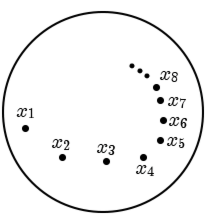
\includegraphics[scale=0.5]{converge.png}
    \caption{An example of a Cauchy Sequence.}
    \label{fig:cauchy_sequence}
  \end{figure}

  What exactly does the above say? Well, in a sense, it says that a Cauchy sequence consists of elements in a metric space that, as the sequence continue, get closer and closer to each other. The first thing to note is that if we have a sequence in our metric space which converges, then the sequence is Cauchy \cite{complete_metric_spaces}. \\

  However, note that a Cauchy sequence need NOT be a convergent sequence!

  \begin{exmp}
  \label{exmp:not_complete}
  For example, take the metric space $X = (0,1]$ with the standard metric and consider the sequence $\{x_n\} \subset X$ given by $x_n = \frac{1}{n}$. While the sequence is Cauchy, the sequence does \textit{not} converge in the space $X$.
  \end{exmp}

  The above motivates the following question: When does Cauchy convergence imply convergence of the sequence? Well, every metric space $X$ will have some Cauchy sequences. If we can prove that all of those Cauchy sequences converge in the space, then we'll have solved the above. This is the reason we have what is called a \textit{complete metric space}.

  \begin{defn}
  A metric space $(X,d)$ is said to be \textit{complete} if it fulfills the above discussed conditions. That is to say, for any Cauchy sequence $\{x_n\} \subset X$, $x_n$ converges in $X$ (ie, converge to a point in $X$).
  \end{defn}

  Now for some examples of complete metric spaces:
  \begin{exmp}
  \label{exmp:rn_complete_metric_space}
  $\mathbb{R}^n$ with the standard metric is a complete metric space. Professor Cliffe Taubes showed this in Lecture 10. Please see the notes \href{https://canvas.harvard.edu/courses/4012/files/1066212/download?wrap=1}{here}. To refresh your memory, the argument had to do with representing each decimal as a decimal expansion!
  \end{exmp}

  We need one more thing about metric spaces before we can continue. For a metric space, we can define the \textit{diameter} of the metric space as follows.
  \begin{defn}
  \label{defn:diameter}
  Let $(X,d)$ be a metric space. Then the diameter of $X$ (noted as diam $X$), is given by:
  $$
    \text{diam } X = \sup \{d(x,y) : x,y \in X \}
  $$
  \end{defn}
  Definition \ref{defn:diameter} is essentially saying the the diameter of a metric space is the maximum distance any two points can be within that metric space. So, on the bounded metric, for any metric space, we know the diameter can be at most $M$. For $\mathbb{R}$ with the standard metric, the diameter is infinite. For Example \ref{exmp:not_complete}, the diameter is $1$ (here, note that because we take the supremum, we're considering the limit points of $X$ too, in a sense).\\

  In relation to metric spaces, we now present an interesting result which we will need later. Note that this is presented as Lemma 48.3 by Munkres \cite{topology_book}.

  \begin{lem}
    \label{lem:nested_sequence}
    Let $C_1 \supset C_2 \supset \cdots$ be a nested sequence of nonempty closed sets in the complete metric space $X$. If diam $C_n \to 0$, then $\bigcap C_n \neq \emptyset$.
  \end{lem}

  What is this saying, exactly? For reference, take a look at Figure \ref{fig:nested} while we discuss the main ideas behind the Proof (for a formal statement of the proof, see Munkres \cite{topology_book}).\\

  Let's simplify a bit and suppose the sets $C_k$ are actually intervals on the real line. The the image looks something like Figure \ref{fig:nested}, where each subsequence interval is ``nested'' within the previous intervals. We want to show that the intersection of all of these closed intervals is non-empty (ie, $\exists p \in \bigcap_i C_i$).\\

  \begin{figure}
  \centering
  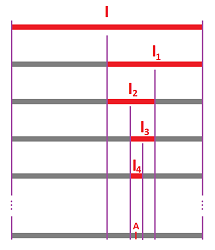
\includegraphics[scale=0.7]{nested.png}
  \caption{Nested Intervals.}
  \label{fig:nested}
  \end{figure}

  What we can do is we can take advantage of the fact that the space is a complete metric space. First, let's try to construct a sequence using the sets that will converge to a specific point contained within all the sets (thereby showing the intersection is non-empty). Well, let's start by picking $x_n \in C_n$ (ie, we pick a point within each nested interval, and these points form our sequence). Notice, immediately, that $d(x_n,x_m) \to 0$ because the intervals are nested, therefore for large enough $N=\max\{n,m\}$, all points are contained within the interval $I_N$, and by assumption, diam $I_N \to 0$! \\

  Therefore, we have a Cauchy sequence. Now using the property that the space $(X,d)$ is a \textit{Complete} \textit{Metric} \textit{Space}, we conclude that this sequence must converge to some point $x_n \to x \in X$. However, note that $x \in \bar{C_k} = C_k$ because the subsequence $x_k \in C_k$ for all $k$. This implies our result!

  \section{Baire spaces}
  Now to the main point of our lecture! We've arrived at Baire spaces. We follow Munkres closely in our presentation, so if anything is confusing, please take some time to reference it \cite{topology_book}.

  \begin{defn}
  \label{defn:baire_space}
  A space $X$ is said to be a \textit{Baire Space} if given any countable collection $\{A_n\}$ of closed sets of $X$ each of which has an empty interior, their union $\bigcup_n A_n$ also has an empty interior in $X$.
  \end{defn}

  Another way to remember Definition \ref{defn:baire_space} is to think about it this way. Baire space ``preserve'' the interior under the operation of union. If all elements have an empty interior, their union has an empty interior. \\

  We can also rephrase the definition a bit to try to get a better understanding. Another way to think of a Baire space is as a space where, if we know that the union of countably subsets has a non-empty interior, then we know that \textit{at least} one of the sets in the union must have a non-empty interior.\\

  Using everything what we learned from Definition \ref{def:dense}, we can reformulate the definition above more succinctly as:
  \begin{defn}
  \label{defn:baire_closed}
  The interior of $\bigcup A_n$ where each $A_n$ is closed nowhere dense is empty.
  \end{defn}

  Even further, thought still equivalent, we can define a Baire space to be a space where:
  \begin{defn}
  \label{defn:baire_open}
  $\bigcap_n A_n$ is dense if all $A_n$ are dense open sets!
  \end{defn}

  Intuitively, Definition \ref{defn:baire_open} is the ``open'' way to define Baire spaces, and Definition \ref{defn:baire_closed} is the ``closed'' way to define Baire spaces. They are equivalent if we recall two facts discussed previously: (1) the complement of an open sets is a closed sets, and (2) the complement of nowhere dense set is a dense set.

  \section{Baire Category Theorem}
  Now that we have a firm grasp of Baire spaces, we can finally prove the Baire Category Theorem (if you would like to know where the term ``category'' comes from, check Munkres \cite{topology_book}).
  For reference, we now restate Theorem \ref{thrm:baire}.
  \begin{thrm}
    \label{thrm:baire2}
  If $X$ is a \textit{compact Hausdorff space} or a \textit{complete metric space}, then $X$ is a \textit{Baire space}.
  \end{thrm}

  \subsection{Compact Spaces}
  Before we can really understand the proof, though, we must first cover another, simpler theorem which has to do with the \textit{finite intersection} property of sets.
  \begin{defn}
  We'll say that a collection $C$ has the finite intersection property if for every finite sub-collection of $C$, the intersection of all of the sets in the sub-collection is non-empty.
  \end{defn}

  How can we think about this? Well, pictures are always worth more than words, so let's try to have a visual for this. We start with a collection of sets C. Imagine these as just a bunch of blobs in some space, for example. Then this collection has the finite intersection property if I can take any finite number of blobs, and they always overlap. Now, this doesn't mean that all of the blobs must overlap! \\

  The following theorem helps us relate the finite intersection property to compact spaces. For reference, recall Definition \ref{defn:compact_spaces}.

  \begin{defn}
  \label{defn:compact_spaces}
  A space $X$ is said to be compact if every open covering $A$ of $X$ contains a finite subcollection that also covers $X$.
  \end{defn}

  \begin{thrm}
  Let X be a topological space. Then X is compact if and only if for every collection C of closed sets in X having the finite-intersection property, the intersection over all elements in the collection is non-empty.
  \end{thrm}

  Instead of an open cover, we have a collection satisfying the finite intersection property. Instead of being able to find a finite sub-cover, we take the intersection and prove it is non-empty. Intuitively, this still measure how tightly packed a space is. Furthermore, we can see that this is similar to our previous understanding of compactness, but instead approaching it from a complementary view point. \\

  What are the steps to proof the above is equivalent to our previous theorem? Well, the two theorems are almost identical, we just have properties of open sets replaced with properties of closed sets. In fact, this gives us an inspiration. Why not just see if we can take complements?\\

  First, let's suppose we're given an arbitrary collection of sets closed sets $\mathcal{C}$ of $X$. Then take the collection consisting of the complements:
  $$
  \mathcal{A} = \{ X - C \mid C \in \mathcal{C}\}
  $$

  So now, we've gone from closed sets to open set! Fantastic. Well, our original theorem also considered open set covers of $X$. Well, you should notice that $\mathcal{A}$ is a covering of $X$ if and only if the intersection of all elements of $\mathcal{C}$ is empty. This follows almost directly from DeMorgan's law

  $$
  X - \bigcup_{\alpha \in J} A_{\alpha} = \bigcap (X - A_{\alpha})
  $$

  If we have a covering of $X$ by $\mathcal{A}$, then the LHS is the empty set. So then the intersection of $\mathcal{C}$ is empty! Intuitively, if you can cover the entire space with the the union of everything that's NOT in the collection $\mathcal{C}$, it must mean there's nothing shared by all the elements of $\mathcal{C}$!\\

  So, the above isn't too bad. However, our original theorem also talks about finite sub-covers. So, let's say there exists a finite sub-collection of $\mathcal{A}$. Then by the similar argument as above, the corresponding complements must share no elements.\\

  Therefore, we now have a way to go from open sets to closed sets, from open covers to empty infinite intersections, and from finite-sub-covers to finite, empty intersections!\\

  Let's revisit our new theorem of compactness. It says that $X$ is compact when ``Given any collection of closed sets, if every finite intersection of elements from this collection is non-empty, then the intersection of all elements is non-empty''. Using the interchangeability of closed and open sets, we can reword this equivalently by saying that ``Given any collection of open sets, if every finite sub-collection of these elements is NOT a cover of X, then the entire collection is NOT a cover''. Notice that we're just replacing the logical equivalents from above, and now we're so close to our original theorem!\\

  What's the last step? Well, the above is in the form $P \implies Q$, which is logically equivalent to $\lnot Q \implies \lnot P$, and this reads: $X$ is compact when ``Given a collection of open sets that covers X, then there is at least one finite sub-collection which also covers X''.\\

  \subsection{The Main Theorem}

  The key aspects of the theorem are the fact the space is either compact Hausdorff or a complete metric space! Why? Well, these types of spaces have very important properties that we can take advantage of to show that the union of sets with an empty interior also has an empty interior (here, we will use the ``open'' definition of a Baire space).
  \begin{enumerate}
    \item Regularity. We've shown before that all metric spaces are regular (see Proposition \ref{prop:metric_spaces_regular}), and the compact Hausdorff spaces are regular \cite{hausdorff_regular}! Regularity is important because we use it to construct a sequence of non-empty, nested sets disjoint from the sets in our union (similar to Urysohns Lemma).
    \item The countable intersection of non-empty, closed, nested sets is non-empty (where diam $C_n \to 0$ if we have a metric space)! We showed this for complete metric spaces in Lemma \ref{lem:nested_sequence}.
    \item We also know this to be the case for compact spaces in general, as discussed previously. Therefore, a sequence of non-empty, nested sets $\{C_n\}$ such that $C_0 \supset C_1, \cdots \supset C_i \cdots$ posses the finite intersection property \cite{finite_intersection}. Then, by compactness of the space $X$, the finite intersection property implies that the intersection must be non-empty. This is of utmost importance because it is what allows us to show the existence of a point in an open set but not in the union of our nowhere dense closed sets.
  \end{enumerate}

  As always, a picture is worth a thousand words, so take note of Figure \ref{fig:baire_category_theorem} while I explain the rest of the theorem.\\

  \begin{figure}
    \centering
    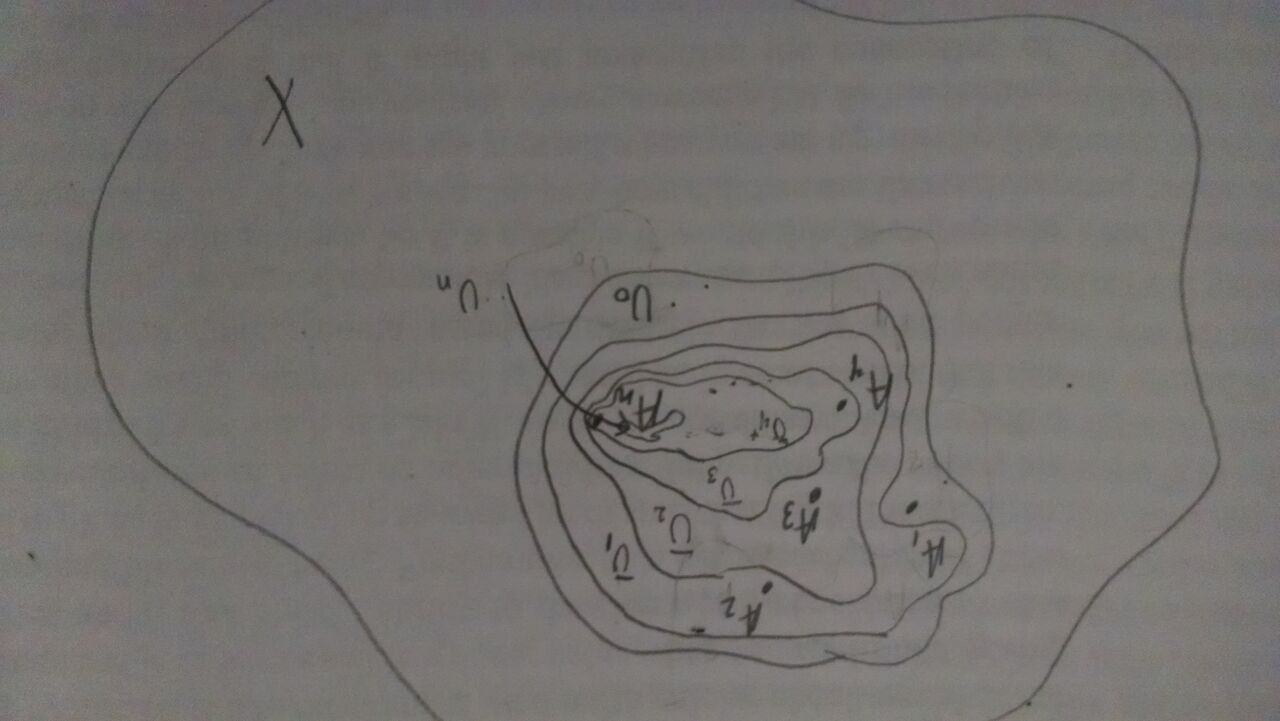
\includegraphics[angle=180,scale=0.2]{baire_theorem_image.jpg}
    \caption{Illustration of the idea behind the proof of Baire's Category Theorem.}
    \label{fig:baire_category_theorem}
  \end{figure}

  The main strategy for showing that the union has an empty interior is to show that the union contains \textbf{no} open sets (other than the empty set)! If the union doesn't contain open sets, then its interior is empty! How can we show an arbitrary open set $U_0$ isn't contained in $\bigcup_n A_n$ for some countable collection? Well, we can just show that there exists a point $p \in U_0$ where $p \notin \bigcup_n A_n$! \\

  We can show this by constructing a sequence of sets from each $A_n$:
  \begin{enumerate}
    \item The set $U_n$ is disjoint from $A_n$ (in fact, its closure is disjoint!). If we look at Figure \ref{fig:baire_category_theorem}, we see that each $U_1$ avoids $A_1$ and so on. We can do this because the space is regular and because the $A_n$ are closed. More formally:
    \begin{align*}
      \bar{U}_n \cap A_n = \emptyset \\
      \bar{U}_n \subset U_{n-1}
    \end{align*}
    Essentially, we can take a look at $U_{n-1}$ and choose a point $y \in U_{n-1}$ (the space is non-empty by induction). Then by regularity of $X$, we can find an open neighborhood of this point $y$ that does not intersect with $A_n$ because $A_n$ is closed (in fact, the closure of this set, call it $U_n$, does not intersect with $A_n$). Additionally, we can have $\bar{U}_n \subset U_{n-1}$ because $U_{n-1}$ is open and $X$ is regular (with additional condition that diam $U_n < \frac{1}{n}$ in the metric space case). These properties of regular spaces are discussed in Lemma 31.1 in Munkres \cite{topology_book}.
  \end{enumerate}

  If we have this sequence, we can then take advantage of the fact the space is compact Hausdorff and/or a complete metric space to claim that there exists a point $p \in \bigcap_n U_n \subset U_0$ which, by construction, is not in \textit{any} of the $A_n$ (thereby proving that the open set $U_0$ cannot be contained in $\bigcup_n A_n$). Figure \ref{fig:baire_category_theorem} makes this clear. As we've shown before, the intersection of all the sets we've created is contained in $U_0$, is non-empty, and does not intersect the union. Therefore, $U_0$ cannot be contained in $\bigcup_n A_n$, implying $\bigcup_n A_n$ has an empty interior.\\

  That's really all there is to it!

  \section{Sample Problem!}
  Now that we understand the theorem, let's try a sample problem. In particular, we'll tackle Problem 2 on page 299 of Munkres.

  \begin{exmp}
  The Baire Category Theorem implies that $\mathbb{R}$ cannot be written as a countable union of closed subsets having empty interiors. Show this fails if the sets are not required to be closed.
  \end{exmp}
  As we discussed in Example \ref{exmp:rn_complete_metric_space}, $\mathbb{R}$ is a complete metric space, therefore it is a Baire space, which implies that it cannot be written as a countable union of closer subsets having empty interiors.

  In the proof, it's obvious that we need the property that the sets are closed in order to create the sets $U_n$. So obviously, the proof we've given won't go through if we drop the closed set assumption.

  However, let's try to give an explicit example to this problem. What we can do, is we can actually consider the set of rational numbers $\mathbb{Q} = \{q_1,q_2, \cdots, q_n, \cdots\}$, and then create the sets that consists of the union of a single rational point with the irrational numbers:
  $$
  A_n = (\mathbb{R} \setminus \mathbb{Q} \cup \{q_n\})
  $$

  We can do this because it is clear that $\mathbb{R} = \bigcup_n A_n$. Furthermore, note that each $A_n$ has an empty interior! (no open interval contains only elements within each $A_n$), or another way to see it, is that $\R \setminus A_n = \Q - \{q_n\}$ is dense in $\R$. However, each $A_n$ is \textit{not} closed. In fact, the set is neither open nor closed, and therefore we can create them only because we've dropped the requirement that each $A_n$ should be closed.\\

  Thanks for coming to lecture! That's all :)

  \section{Appendix}
  In this section, I describe some more technical aspects quickly discussed in the lecture above.
  \begin{prop}
  \label{prop:pi_n_irrational}
  We want to show that $\forall n > 1$, $\frac{\pi}{n}$ is irrational. We do this by contradiction. Suppose it where the case that $\frac{\pi}{n}$ is rational. Then we can express $\frac{\pi}{n} = \frac{p}{q}$ where $p,q \in \mathbb{Z}$. Therefore, we can rearrange the above equation to have $\pi = \frac{np}{q} = \frac{p'}{q}$ where $p' \in \mathbb{Z}$. This is a contradiction on the fact that $\pi$ is irrational.
  \end{prop}

  \begin{prop}
  \label{prop:sum_rational_irrational}
  Let $x \in \mathbb{Q}$ and $y \in \mathbb{R} \setminus \mathbb{Q}$. Then we claim that $x + y \in \mathbb{R}\setminus \mathbb{Q}$. We prove this by contradiction. Suppose that $x + y \in \mathbb{Q}$, then we can express the sum as a fraction $x + y = \frac{p}{q}$ where $p,q \in \mathbb{Z}$ with $q \neq 0$. Then note that $x = \frac{p'}{q'}$ ($q' \neq 0$ because $x \in \mathbb{Q}$. Therefore, we have that:
  $$
  y = \frac{p}{q} - \frac{p'}{q'} = \frac{pq' - p'q}{pq'}
  $$
  Note that $pq' = p'q \in \mathbb{Z}$ and $pq' \in \mathbb{Q}$, therefore this is a contradiction on the fact that $y$ is irrational.
  \end{prop}

  \begin{prop}
  \label{prop:metric_spaces_regular}
  We proof that all metric spaces are normal, and therefore they are regular (as required by the Baire category theorem).\\
  Suppose we have two closed subsets $A,B$ of a metric spaces $(X,d)$. Then create the sets $U = \{x \in X \mid d(x,A) < d(x,B)\}$ and $V = \{x \in X \mid d(x,B) < d(x,A)\}$. Intuitively, the first is the set of points closer to $A$ than to $B$, and the second the set of points closer to $B$ then to $A$. By construction, $U,V$ are disjoint (strict inequality), each contain $A,B$ respectively, and are open.
  \end{prop}

\begin{thebibliography}{9}
\bibitem{topology_book}
\textit{Topology} by James. R Munkres, Second Edition

\bibitem{metric_spaces}
UC Davis: Metric spaces. Link: \href{https://www.math.ucdavis.edu/~hunter/m125a/intro_analysis_ch7.pdf}{https://www.math.ucdavis.edu/\~hunter/m125a/intro\_analysis\_ch7.pdf}

\bibitem{template}
Template used for these lecture notes can readily be found here: \href{https://github.com/snario/notes-template}{https://github.com/snario/notes-template}. Small modifications were made in the interest of clarity.

\bibitem{wikipedia:dense_set}
Dense Sets. Link: \href{https://en.wikipedia.org/wiki/Dense_set}{https://en.wikipedia.org/wiki/Dense\_set}

\bibitem{overflow:dense_sets}
Understanding the Definition of Dense Sets. Link: \href{http://math.stackexchange.com/questions/58709/understanding-the-definition-of-dense-sets}{http://math.stackexchange.com/questions/58709/understanding-the-definition-of-dense-sets}

\bibitem{dedekind_cuts}
Dedekinda Cuts by Rich Schwartz, \textit{Brown University}. Direct link: \href{http://www.math.brown.edu/~res/INF/handout3.pdf}{http://www.math.brown.edu/~res/INF/handout3.pdf}.

\bibitem{cantor_set}
Cantor Set. Link: \href{https://en.wikipedia.org/wiki/Cantor_set}{https://en.wikipedia.org/wiki/Cantor\_set}

\bibitem{complete_metric_spaces}
Complete Metric spaces. Link: \href{http://pioneer.netserv.chula.ac.th/~lwicharn/2301631/Complete.pdf}{http://pioneer.netserv.chula.ac.th/~lwicharn/2301631/Complete.pdf}

\bibitem{hausdorff_regular}
Compact Hausdorff Implies Normal. Link: \href{http://topospaces.subwiki.org/wiki/Compact_Hausdorff_implies_normal}{http://topospaces.subwiki.org/wiki/Compact\_Hausdorff\_implies\_normal}

\bibitem{finite_intersection}
Finite Intersection Property. Link: \href{https://en.wikipedia.org/wiki/Finite_intersection_property}{https://en.wikipedia.org/wiki/Finite\_intersection\_property}

\end{thebibliography}

  %%%%%%%%%%%%%%%%%%%%%%%%%%%%%%%%%%%%%%%%%%%%%%%
  \end{document}